\section{Моделирование движения двух космических аппаратов как двух материальных точек при действии тяги на одном из них}
\label{SEC:2SPH}

В этом разделе рассмотрим случай, в котором расстояние $a$ между пассивным и активным аппаратами изменяется за счет тяги на активном аппарате.
Аппараты представлены материальными точками, между которыми происходит электростатическое взаимодействие.

\begin{figure}[H]
	\center{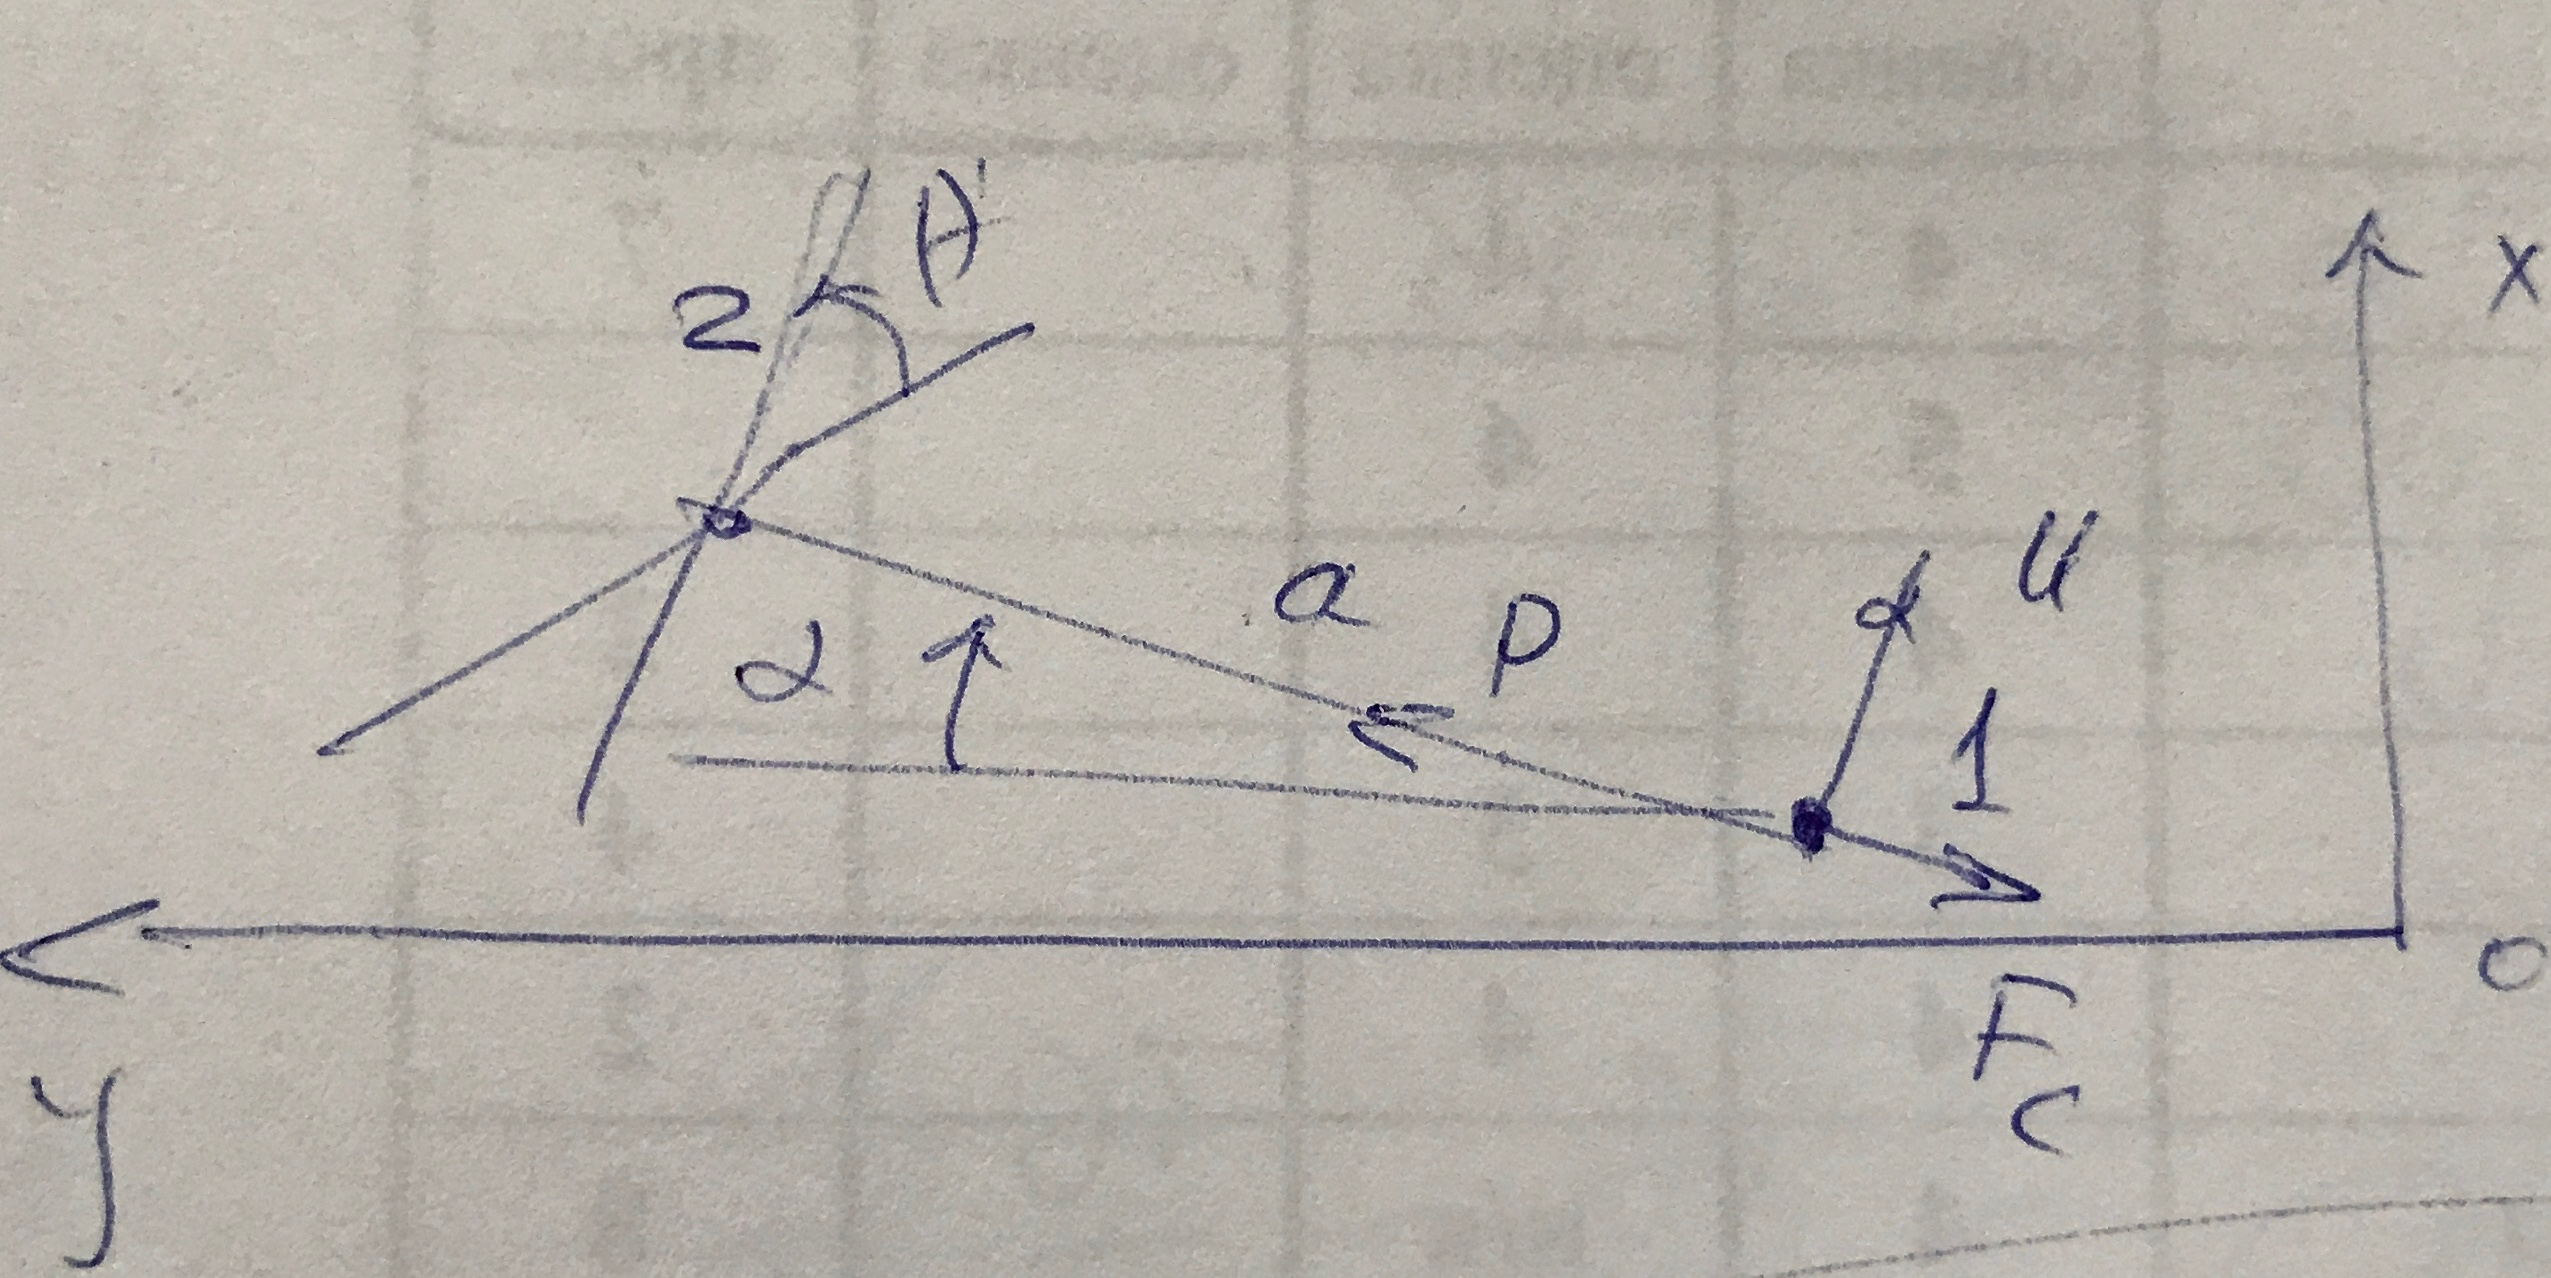
\includegraphics[scale=0.15]{2sph.jpg}}
	\caption{Замена космических аппаратов двумя материальными точками}
	\label{ris:3sph}
\end{figure}

